\documentclass[11pt]{article}
\usepackage[margin=1.05in]{geometry}
\usepackage[T1]{fontenc}
\usepackage{lmodern}
\usepackage{amsmath,amssymb,amsthm,graphicx,booktabs,listings,xcolor,upquote}
\usepackage[hidelinks]{hyperref}

\newtheorem{theorem}{Theorem}\newtheorem{proposition}[theorem]{Proposition}\newtheorem{corollary}[theorem]{Corollary}
\newtheorem{lemma}[theorem]{Lemma}
\theoremstyle{remark}\newtheorem{remark}[theorem]{Remark}
\newcommand{\Sym}{\mathrm{Sym}}\newcommand{\dH}{d_H}\newcommand{\F}{\mathbb{F}}\newcommand{\Z}{\mathbb{Z}}
\newcommand{\Id}{\mathrm{Id}}\newcommand{\Tr}{\operatorname{Tr}}
\lstset{basicstyle=\ttfamily\scriptsize,breaklines=true,columns=fullflexible,keepspaces=true,frame=none,upquote=true}
\title{\bfseries The permutation coboundary constant of the complete complex is $k/3$\\[4pt]
\large for every $k\ge4$, including the powers of two, with four Hamming-native readings that do not obstruct}
\author{Jeromie Beasley}
\date{Version 8, 8 October 2026\\[10pt]
\includegraphics[width=.30\textwidth]{ai_reviewer_advisory.png}}
\emergencystretch=3em
\begin{document}\maketitle
\begin{abstract}
Let $K_k$ be the complete two-dimensional complex on $k$ vertices and let $h_1(K_k,\Sym)$ be its first coboundary expansion constant with permutation coefficients in the normalised Hamming metric, in the convention that counts cells. Chapman and Lubotzky prove $h_1(K_k,\Sym)\ge k/3$ for every $k$ and every permutation degree. We show that this bound is an equality for every $k\ge4$, attained by cochains with values in $\Sym(3)$. For $\F_2=\Sym(2)$ coefficients Kozlov proves the constant is $k/3$ whenever $k$ is not a power of two; it is strictly larger at $k=4$ (where it is $2$) and at $k=8$ (where it is $20/7$), and at larger powers of two it lies between $k/3$ and $k/3+4k/(3(k^2-8))$, with strictness open. The permutation constant reaches the bound at every power of two. At $k=4$ the contrast is sharp: among the subgroups of $\Sym(3)$, the binary subgroup $\F_2$ gives $2$, the cyclic subgroup $\Z/3$ gives $3/2$, and only $\Sym(3)$ itself reaches $4/3$. The proof has three parts. At $k=4,\dots,8$ an explicit witness is computed in integers, checked by two independent programs, and its gauge minimum is kernel-checked in Lean; at $k=4$ the minimum also has a short hand proof, and the attaining cochain is a single triangle carrying the three distinct transpositions of $\Sym(3)$. A balanced replication of a cochain multiplies its triangle defect by $q^3$ and its gauge minimum by exactly $q^2$, so the $k=4$ seed reaches $k/3$ at every multiple of four; the lower bound is proved in full and is an equality of averages, so a cochain attains $k/3$ exactly when every star gauge is optimal. At the remaining $k$, Kozlov's binary witness embeds through one transposition, and a parity retraction shows that no $\Sym(3)$ gauge does better. The replication law, for every cochain, every $k$ and every $q$, and the retraction, for every $k$, are themselves kernel-checked in Lean, so the gauge minimum $6q^2$ of the replicated seed is a kernel-checked fact at every multiple of four. The same value holds in Chapman--Lubotzky's cross-degree convention. The all-$k$ theorem is proved, not searched for: computation supplies explicit witnesses only at $k\le8$, and the proof does not depend on the open question of whether $\F_2$ reaches $k/3$ at the larger powers of two. Four further readings of the same metric are recorded because their content is exact: a regularised twisted torsion that is Lipschitz in Hamming distance on the padded family; the displacement Gram of a permutation, which is half the Laplacian of its cycle graph, sums over a family to half the Laplacian of the Schreier graph of the action, and has a fixed-scale entropy that vanishes exactly on involutions and is bounded by $h(\dH/2)$ for every permutation, with a finite-size deficit given exactly by a lattice sum whose $\ell^3$-scaled limits are $2\zeta(3)$ on even cycles and $\zeta(3)/4$ on odd ones, with every further correction an odd zeta value; an exact embedding of the Hamming metric as a squared distance between graph-subspace projectors, equivalent with explicit constants to Grassmannian geodesic distance; and a fixed-probe response that reads the spectral measure seen by the probe and so separates isospectral defects. None of them obstructs approximation. Grades: [T] derived, [V] computed, [L] kernel-checked in Lean, [C] cited.
\end{abstract}

\section{Setting and conventions}
Two permutations of $n$ points are compared by the fraction of points on which they differ,
$\dH(\sigma,\tau)=\tfrac1n\#\{i:\sigma(i)\ne\tau(i)\}$, a bi-invariant metric on $\Sym(n)$. Following Chapman--Lubotzky \cite{CL1,CL2}, a 1-cochain $\alpha$ on a finite 2-complex $X$ assigns a permutation to each oriented edge with $\alpha(v,u)=\alpha(u,v)^{-1}$; its coboundary on a triangle is the holonomy $\delta\alpha(u,v,w)=\alpha(u,v)\alpha(v,w)\alpha(w,u)$; $\|\delta\alpha\|$ is the mean over triangles of $\dH(\delta\alpha(\Delta),\Id)$; and $d(\alpha,B^1)$ is the least mean over edges of the distance to a coboundary $\delta\beta(u,v)=\beta(u)^{-1}\beta(v)$. The first coboundary Cheeger constant is
\[
h_1^{\rm norm}(X,\Sym)=\min_{\alpha\notin B^1}\frac{\|\delta\alpha\|}{d(\alpha,B^1)},\qquad h_1^{\rm count}(X,\Sym)=\frac{|T|}{|E|}\,h_1^{\rm norm}(X,\Sym),
\]
the first with uniform probability on cells, the second counting cells. On the complete complex $|T|/|E|=(k-2)/3$, so $k/(k-2)$ in the first convention is $k/3$ in the second. The tables use the counting convention, which is the one the enumerations compute and the one in which the $\F_2$ literature states its results. Chapman--Lubotzky define the constant with distance to the cocycles $Z^1$; on the complete complex $H^1$ vanishes and the two agree \cite[Cor.~4.1]{CL2}. For a cochain $\alpha$ we write $N(\alpha)$ for the total triangle defect and $D(\alpha)$ for the gauge minimum, both counted in moved points; with values in $\Sym(3)$ these are integers and $h_1^{\rm count}=\min N/D$ over non-coboundaries.

Since $\Sym(2)\cong\F_2$ and $\dH$ on two points is the discrete metric, the $\F_2$ coboundary expansion constant of Linial--Meshulam \cite{LM} is the $\Sym(2)$ column of the permutation theory, and $h_1(X,\Sym)\le h_1(X,\F_2)$ always \cite[footnote 2]{CL2}. Two conventions for $\Sym$ are in use, and they are kept apart here. In the \emph{same-degree} convention a cochain and the coboundaries it is compared with all take values in one $\Sym(n)$; write $h_1^{\rm same}$. In Chapman--Lubotzky's convention $\Sym$ is the disjoint union of all $\Sym(m)$, and a permutation $\sigma$ of degree $n$ is compared with $\tau$ of degree $m$ by the distance with errors
\[
d(\sigma,\tau)=1-\frac{\#\{j<\min(n,m):\sigma(j)=\tau(j)\}}{\max(n,m)},
\]
which is $\dH$ when $n=m$; write $h_1^{\rm err}$, where the comparison coboundary may have any degree. Sections~\ref{sec:bound}--\ref{sec:all} work in $h_1^{\rm same}$, and Proposition~\ref{prop:crossdeg} shows that both constants are $k/3$ on $K_k$. Where the convention does not matter we write $h_1(K_k,\Sym)$.

The question comes from an earlier attempt to extract an obstruction to soficity from operator data after Astra's non-sofic group of 1 August 2026 \cite{trace}. There the Exel--Loring winding of an almost-commuting pair \cite{EL} was gated numerically and found to be integral and rigid, but rigid in the operator norm: changing a permutation on $\varepsilon n$ points costs $\varepsilon$ in normalised Hamming distance but an amount of order one in operator norm ($2$ for a transposition, $\sqrt3$ for a 3-cycle), so that winding jumps under exactly the local surgery soficity forgives. The lesson was to stop fighting the metric from outside and to study quantities native to it. The coboundary constant of the complete complex is the first calibration in that programme, and Section~\ref{sec:readings} records what the other native readings do.

\section{The bound}\label{sec:bound}
\begin{proposition}[Chapman--Lubotzky {\cite[Prop.~3.2]{CL2}}; T]\label{prop:cl}
For every 1-cochain $\alpha$ on $K_k$ with coefficients in any group carrying a bi-invariant metric,
\[
\frac1k\sum_{x}\|\delta\beta_x-\alpha\|=\frac{k-2}{k}\,\|\delta\alpha\|,
\]
where $\beta_x$ is the star gauge at $x$ defined below and $\|\delta\beta_x-\alpha\|$ is the mean over edges of $\dH(\alpha(e),\delta\beta_x(e))$. Hence $d(\alpha,B^1)\le\frac{k-2}{k}\|\delta\alpha\|$, in counting variables $D\le 3N/k$, and $h_1^{\rm count}(K_k,\Sym)\ge k/3$ for every $k$ and every permutation degree.
\end{proposition}
\begin{proof}
Fix a vertex $x$ and put $\beta_x(x)=\Id$, $\beta_x(u)=\alpha(x,u)$ for $u\ne x$. On a star edge, $\delta\beta_x(x,u)=\beta_x(x)^{-1}\beta_x(u)=\alpha(x,u)$, so the star edges cost nothing. On an edge $(u,v)$ with $u,v\ne x$, bi-invariance and $\alpha(x,v)^{-1}=\alpha(v,x)$ give
\[
\dH\big(\alpha(u,v),\,\alpha(x,u)^{-1}\alpha(x,v)\big)=\dH\big(\alpha(x,u)\alpha(u,v)\alpha(v,x),\,\Id\big)=\dH\big(\delta\alpha(x,u,v),\Id\big).
\]
So after the star gauge at $x$ each non-star edge carries exactly the holonomy of the one triangle it spans with $x$. The cost of a holonomy does not depend on the base point or the orientation, because changing either replaces it by a conjugate or an inverse and $\dH(\cdot,\Id)$ is invariant under both. Summing over $x$, every triangle is counted once for each of its three vertices:
\[
\sum_x\|\delta\beta_x-\alpha\|=\frac1{|E|}\sum_x\sum_{\substack{u<v\\u,v\ne x}}\dH(\delta\alpha(x,u,v),\Id)=\frac{3|T|}{|E|}\,\|\delta\alpha\|=(k-2)\,\|\delta\alpha\|,
\]
using $|T|/|E|=(k-2)/3$. Dividing by $k$ gives the identity. The least of the $k$ star costs is at most their mean, so $d(\alpha,B^1)\le\frac{k-2}{k}\|\delta\alpha\|$; in moved points the same count reads $\sum_x\mathrm{cost}(\beta_x)=3N$ and $D\le 3N/k$.
\end{proof}
The identity is an equality of averages, not an estimate, and it also says when the bound is met.
\begin{corollary}[The equality case; T]\label{cor:equality}
A cochain $\alpha\notin B^1$ has $N/D=k/3$ if and only if every star gauge $\beta_x$ is an optimal gauge for $\alpha$.
\end{corollary}
\begin{proof}
Each star cost is at least $D$ and their mean is $3N/k$. So $D=3N/k$ holds exactly when no star cost exceeds $D$.
\end{proof}
Every witness of Sections~\ref{sec:small} and~\ref{sec:all} is therefore a cochain all of whose star gauges are optimal. Script \texttt{K3-V4-STAR} checks this on every witness of Appendix~\ref{sec:witnesses}.

\begin{remark}[Bi-invariance is the hypothesis; V]
Replacing $\dH$ by a site-weighted Hamming metric, still a metric but no longer bi-invariant, moves the ratio of Proposition~\ref{prop:cl} off $(k-2)/k$ at once: at $k=4$ the weighted ratio ranges over $0.486$--$0.548$ against an exact $0.500$, with the same drift at $k=5,6$.
\end{remark}

\section{The bound is attained at \texorpdfstring{$k=4,\dots,8$}{k=4..8}: computed witnesses}\label{sec:small}
\begin{theorem}[T+V+L]\label{thm:small}
For $k=4,5,6,7,8$, $h_1^{\rm count}(K_k,\Sym)=k/3$ and $h_1^{\rm norm}(K_k,\Sym)=k/(k-2)$, attained by a cochain with values in $\Sym(3)$. The values of the coefficient subgroups are
\begin{center}
\begin{tabular}{lccccc}\toprule
$h_1^{\rm count}$ & $k=4$ & $k=5$ & $k=6$ & $k=7$ & $k=8$\\\midrule
$\Sym(2)=\F_2$ & $2$ & $5/3$ & $2$ & $7/3$ & $20/7$ \\
$\Sym(3)$ & $4/3$ & $5/3$ & $2$ & $7/3$ & $8/3$\\
lower bound $k/3$ & $4/3$ & $5/3$ & $2$ & $7/3$ & $8/3$\\\bottomrule
\end{tabular}
\end{center}
The $\F_2$ row is Meshulam--Wallach and Kozlov \cite{MW,Koz}, including Kozlov's value $8/3+4/21=20/7$ at $k=8$; the $\Sym(3)$ row is this paper.
\end{theorem}
\begin{proof}
The lower bound is Proposition~\ref{prop:cl}. For the upper bound one cochain per $k$ suffices, provided its ratio is computed exactly and its gauge minimum is the true minimum over all gauges. With $\Sym(3)$ coefficients every Hamming distance is $0$, $2/3$ or $1$, so all quantities are moved-point counts in integers and ``$=k/3$'' is rational equality. The gauge minimum is taken over all $6^{k-1}$ gauges with $\beta(\text{root})=\Id$, which loses nothing because a constant right factor conjugates every edge term and the moved-point count is conjugation-invariant. The witnesses are listed in Appendix~\ref{sec:witnesses}; their triangle defects and gauge minima are
\[
\begin{array}{c|ccccc}
k&4&5&6&7&8\\\hline N/D & 8/6 & 10/6 & 36/18 & 28/12 & 72/27
\end{array}
\]
and each equals $k/3$. Every witness was recomputed by a second program sharing no code with the search (Appendix~\ref{sec:gates}), which returned the same $N$, the same $D$ and the same minimising gauge. The same five equalities are kernel-checked in Lean (Section~\ref{sec:lean}).
\end{proof}

\begin{figure}[t]\centering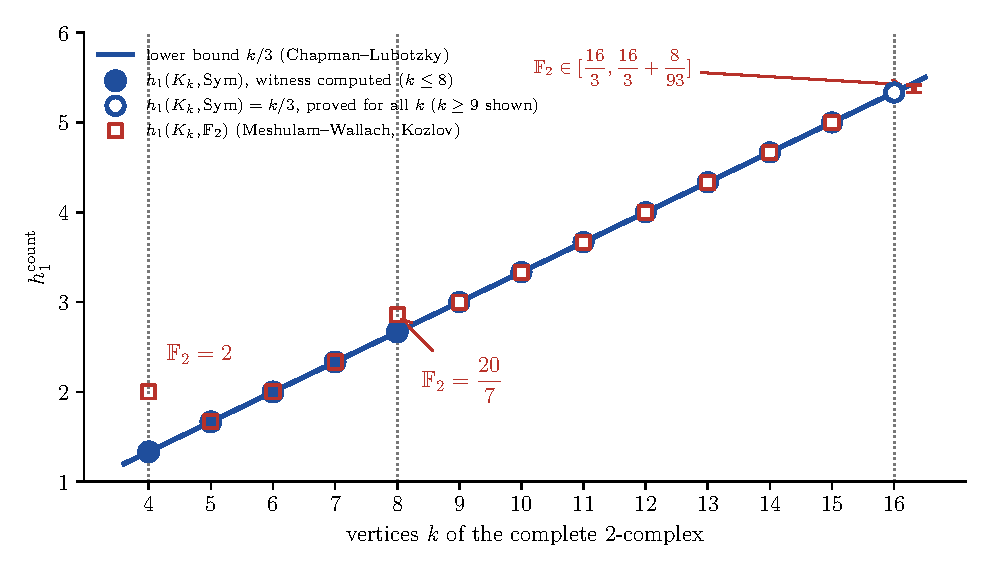
\includegraphics[width=.9\textwidth]{fig_ladder_v4.pdf}
\caption{The bound and the constant. The permutation constant sits on $k/3$ at every $k$: computed and kernel-checked for $k\le8$ (filled), proved by Theorem~\ref{thm:all} for every $k$ (open). The $\F_2$ constant is above the bound at $k=4$ ($2$) and $k=8$ ($20/7$); at $k=16$ Kozlov's bounds confine it to the bracketed interval $[16/3,\,16/3+8/93]$, and whether it lies strictly above $16/3$ is open.}\end{figure}

\subsection{The four-vertex seed has a hand proof}
\begin{proposition}[$k=4$; T+V]\label{prop:k4}
Let $\alpha$ be the identity on the three edges at vertex $0$ and carry the three distinct transpositions $a,b,c$ of $\Sym(3)$ on the edges $12,13,23$. Then $N(\alpha)=8$ and $D(\alpha)=6$, so $N/D=4/3=k/3$. Over all $\Sym(3)$-cochains on $K_4$ the minimum ratio is $4/3$; restricted to $\Sym(2)$ it is $2$, and restricted to $\Z/3$ it is $3/2$.
\end{proposition}
\begin{proof}
All four triangle holonomies are transpositions, so $N=8$; the identity gauge costs $6$. Suppose a gauge cost less than $6$. Every non-identity residual edge costs at least $2$, so at most two edges are non-identity. Every triangle has odd holonomy, so the residual must place a transposition on every triangle: a single transposition meets only two of the four triangles, and two transpositions sharing a vertex leave the opposite triangle even. Hence the residual is two transpositions on a perfect matching, with no budget for a 3-cycle. But then the two triangles containing the matching edge at vertex $0$ have equal holonomy based at $0$, whereas the three triangle holonomies of $\alpha$ based at $0$ are $a,b,c$, all distinct, and a gauge conjugates all three by the same permutation, which preserves distinctness. So $D=6$. The minimum $4/3$ over all $\Sym(3)$-cochains then needs no search: Proposition~\ref{prop:cl} bounds every ratio below by $4/3$, and $\alpha$ attains it. Only the subgroup minima, $2$ for $\Sym(2)$ and $3/2$ for $\Z/3$, come from exhausting all $6^6$ cochains on $K_4$ [V].
\end{proof}
The mechanism is non-abelian. The product of the three distinct transpositions around the triangle is a transposition, while each adjacent product is a 3-cycle (kernel-checked as \texttt{k4\_mechanism}). A single transposition on one edge ($\F_2$) pays $2$ on each of the two triangles through it against a gauge cost of $2$, ratio $2$; two 3-cycles pay $3$ on two triangles against gauge cost $4$, ratio $3/2$. Only three \emph{different} involutions reach the bound.

\begin{figure}[t]\centering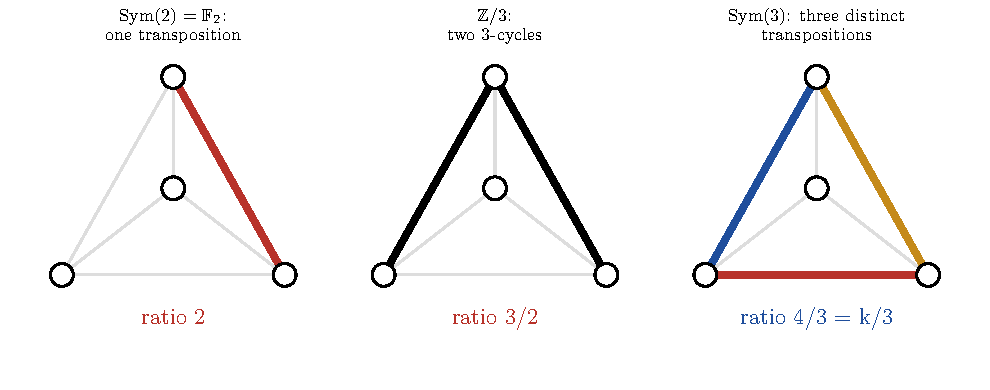
\includegraphics[width=.95\textwidth]{fig_k4.pdf}
\caption{$k=4$ by coefficient subgroup. The bound needs the non-abelian group, not a larger abelian one.}\end{figure}

\subsection{The other computed witnesses}
At $k=5,6,7$ the $\F_2$ theory already reaches $k/3$ by Kozlov's theorem, and the witnesses found are the $\F_2$ ones at $k=5$ (a path on four vertices) and $k=7$ (a four-cycle with two pendant edges), both carrying a single transposition. At $k=6$ the witness found gauges to six 3-cycles, a $\Z/3$-valued cochain. At $k=8$ the witness, gauged to its minimising coboundary, has residual support on 13 of the 28 edges: twelve transpositions, using all three transpositions of $\Sym(3)$, and one 3-cycle (Figure~\ref{fig:w8}). A cochain valued in a single transposition is an $\F_2$ cochain, and $\F_2$ cannot reach $8/3$ at $k=8$, so this witness must use more of $\Sym(3)$. Section~\ref{sec:all} gives a second, simpler $k=8$ witness with $(N,D)=(64,24)$ and twelve transposition edges.

\begin{figure}[t]\centering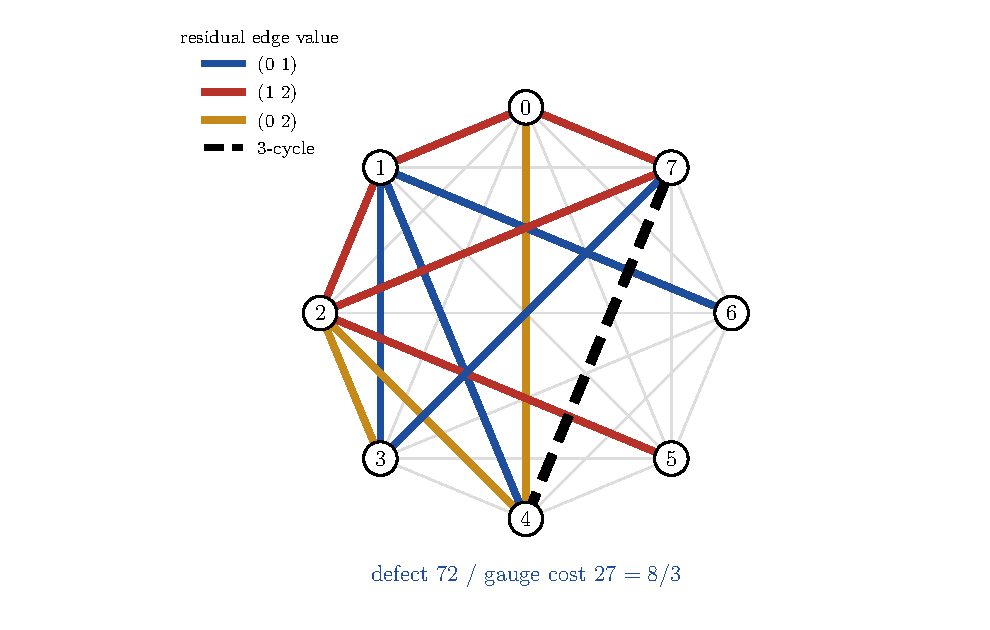
\includegraphics[width=.8\textwidth]{fig_witness8.pdf}
\caption{The $(72,27)$ witness at $k=8$ after gauging: 13 of 28 edges non-identity, grey edges the identity.}\label{fig:w8}\end{figure}

\subsection{What the search is and is not}
The witnesses at $k=5,\dots,8$ were found by simulated annealing over cochains, with the exhaustive gauge minimum recomputed exactly at every step (the $6^{k-1}$-entry cost vector is updated incrementally when one edge changes). A search that returns $k/3$ is a proof, because an upper-bound witness has met a proven lower bound. A search that does not is nothing: at $k=8$ one annealing seed reached $8/3$ at restart 13 (counting from 0) while a second stalled at $87/32$ through twenty-two restarts, and earlier hill climbs without incremental updates stalled at $31/11$. Exhaustion over cochains is available only at $k=4$: $K_5$ already carries $6^{10}\approx6.0\times10^7$ cochains and $K_6$ carries $6^{15}\approx4.7\times10^{11}$, while $K_{16}$ has $6^{15}$ gauges for each cochain. Past $k=8$ the proof proceeds by construction.

\section{The bound is attained for every \texorpdfstring{$k\ge4$}{k>=4}}\label{sec:all}
\begin{lemma}[Balanced replication; T+L]\label{lem:rep}
Replace each vertex $i$ of $K_k$ by a cluster of $q\ge1$ vertices $(i,a)$. Put the identity on every edge inside a cluster and $\alpha_{ij}$ on every edge from cluster $i$ to cluster $j$; call the resulting cochain $\alpha^{[q]}$ on $K_{qk}$. Then, for any coefficient group with a bi-invariant metric,
\[
N(\alpha^{[q]})=q^3N(\alpha),\qquad D(\alpha^{[q]})=q^2D(\alpha),\qquad\text{so}\qquad \frac{N(\alpha^{[q]})}{D(\alpha^{[q]})}=q\,\frac{N(\alpha)}{D(\alpha)}\ \ (\alpha\notin B^1).
\]
This is an exact scaling law for every cochain, not only for extremisers.
\end{lemma}
\begin{proof}
A triangle with vertices in three distinct clusters carries the holonomy of the underlying triangle of $K_k$, and each triangle of $K_k$ has $q^3$ such lifts. A triangle with two vertices in one cluster carries $\Id\cdot\alpha_{ij}\cdot\alpha_{ij}^{-1}=\Id$, and a triangle inside one cluster carries $\Id$. This gives the numerator.

For the denominator take an arbitrary gauge $\beta_{(i,a)}$ on $K_{qk}$, with no assumption that it is constant on clusters. A \emph{section} is a choice of one representative $A_i\in\{1,\dots,q\}$ in each cluster; there are $q^k$ of them. Each section gives a gauge $\gamma^A_i=\beta_{(i,A_i)}$ on $K_k$, whose cost is at least $D(\alpha)$ by definition of $D$. An inter-cluster edge $((i,a),(j,b))$ is used by exactly the sections with $A_i=a$ and $A_j=b$, and there are $q^{k-2}$ of those. Summing the costs of all sections therefore counts every inter-cluster edge of $K_{qk}$ exactly $q^{k-2}$ times:
\[
q^k\,D(\alpha)\;\le\;\sum_{A}\mathrm{cost}(\gamma^A)\;=\;q^{k-2}\sum_{i<j}\sum_{a,b}\dH\big(\beta_{(i,a)}^{-1}\alpha_{ij}\beta_{(j,b)},\Id\big)\;=\;q^{k-2}\,\mathrm{cost}_{\rm inter}(\beta).
\]
So the inter-cluster cost of $\beta$ is at least $q^2D(\alpha)$, and since the intra-cluster cost is non-negative, every gauge costs at least $q^2D(\alpha)$. This is a finite double count; no probability and no averaging over an infinite set is used. Conversely, copying an optimal gauge of $\alpha$ across each cluster costs nothing inside clusters and exactly $q^2D(\alpha)$ between them. For an infinite coefficient group, use near-optimal gauges and take the infimum.
\end{proof}

\begin{corollary}[Every multiple of four; T+V+L]\label{cor:mult4}
For $k=4q$ the replicated seed of Proposition~\ref{prop:k4} has $N=8q^3$ and $D=6q^2$, so $N/D=4q/3=k/3$. It has exactly $3q^2$ non-identity edges, all transpositions, and uses only permutation degree three.
\end{corollary}
At $q=2$ the replicated $K_8$ has $(N,D)=(64,24)$, confirmed by exhausting all $6^7$ root-fixed gauges. For every $q$ the lemma and the corollary are kernel-checked (\texttt{rep\_defect}, \texttt{rep\_attain}, \texttt{rep\_lower}, \texttt{rep\_seed}; Section~\ref{sec:lean}), the lower bound through the same count over the $q^k$ sections, with no assumption that the gauge is constant on clusters. Beyond that the minima are values of the lemma, not enumerations: the defects counted explicitly are $N=216,512,4096,32768$ at $k=12,16,32,64$, against lemma minima $D=54,96,384,1536$.

\begin{figure}[t]\centering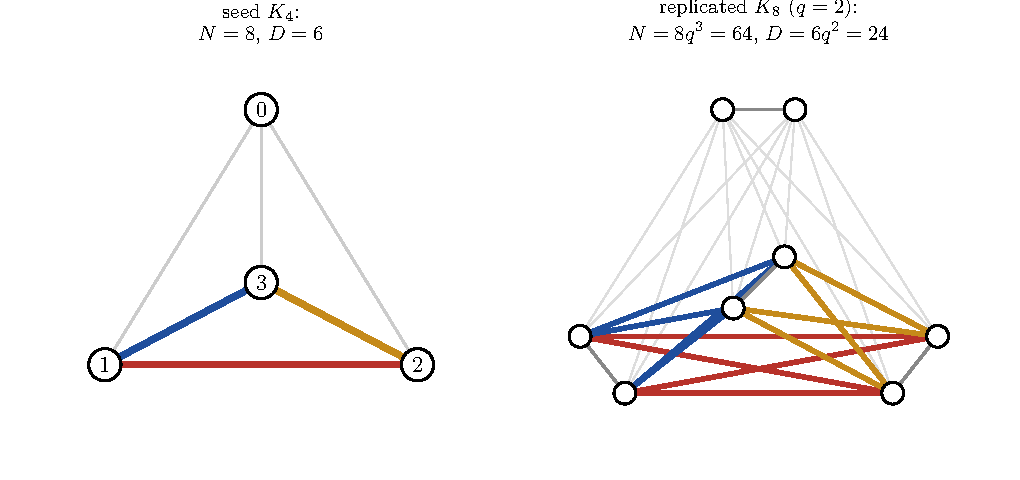
\includegraphics[width=.95\textwidth]{fig_replication.pdf}
\caption{Balanced replication. Each vertex of the $k=4$ seed becomes a cluster of $q$ vertices joined by identity edges (grey); each coloured seed edge becomes the $q^2$ edges between two clusters. Triangles across three clusters copy the seed holonomy, triangles with two vertices in one cluster close to the identity, and the gauge minimum scales exactly by $q^2$.}\label{fig:rep}\end{figure}

\begin{theorem}[T]\label{thm:all}
For every $k\ge4$,
\[
h_1^{\rm count}(K_k,\Sym)=\frac k3,\qquad h_1^{\rm norm}(K_k,\Sym)=\frac{k}{k-2},
\]
and the minimum is attained by a cochain with values in $\Sym(3)$.
\end{theorem}
\begin{proof}
The lower bound is Proposition~\ref{prop:cl}. If $k$ is a multiple of four, Corollary~\ref{cor:mult4} gives a witness; this covers every power of two $\ge4$. Otherwise $k$ is not a power of two and Kozlov proves $h_1^{\rm count}(K_k,\F_2)=k/3$ \cite[Thm.~4.2, Cor.~4.3]{Koz}. Embed the binary group as $H=\{\Id,t\}$ for one transposition $t$ of $\Sym(3)$ and read Kozlov's witness as an $H$-valued cochain. Counted in moved points, numerator and denominator are both twice their binary values, since a transposition moves two points (in normalised units the common factor is $2/3$); either way the ratio is unchanged when gauges range over $H$. Gauges outside $H$ do no better. The retraction $r:\Sym(3)\to H$, $r(g)=t^{\operatorname{parity}(g)}$, is a homomorphism that restricts to the identity on $H$, and it does not increase the moved-point count: an even element goes to $\Id$ at cost $0$, and an odd element is a transposition of cost $2$ and goes to $t$ at cost $2$. For an $H$-valued cochain $\alpha$ and any $\Sym(3)$-gauge $\beta$, the edge term $r(\beta_u^{-1}\alpha_{uv}\beta_v)=r(\beta_u)^{-1}\alpha_{uv}\,r(\beta_v)$ is the edge term of the $H$-gauge $r\circ\beta$ and costs no more. So the $\Sym(3)$ gauge minimum equals the $H$ gauge minimum, and the ratio is $k/3$.
\end{proof}
\begin{remark}[What each part rests on]
The lower bound $k/3$ is Chapman--Lubotzky's star average \cite[Prop.~3.2]{CL2}, proved in Section~\ref{sec:bound} [T]; it is not formalised for general $k$. Equality at $k=4,\dots,8$ is by explicit $\Sym(3)$ witnesses whose gauge minima are kernel-checked [V+L]. Equality at every multiple of four is the balanced replication of the $k=4$ seed, kernel-checked for every $q$ [T+L]. Equality at the remaining $k$ is Kozlov's binary witness [C] together with the parity retraction, which is kernel-checked for every $k$ [T+L]. Kozlov's theorem and the assembly of the three cases into Theorem~\ref{thm:all} are not in the Lean library.
\end{remark}
For comparison, Kozlov's results at the powers of two are exact at the two smallest cases, $h_1^{\rm count}(K_4,\F_2)=2$ and $h_1^{\rm count}(K_8,\F_2)=20/7$, and for $k=2^d$ with $d\ge3$ the doubled staircase gives
\[
\frac k3\le h_1^{\rm count}(K_k,\F_2)\le\frac k3+\frac{4k}{3(k^2-8)}
\]
\cite[Thm.~4.6]{Koz}, so $16/3+8/93$ at $k=16$ and $32/3+16/381$ at $k=32$. Whether the excess is strict at every power of two is open, and nothing above uses it.

\begin{remark}[Which coefficient subgroup is needed; T+C]
For $k$ not a power of two the binary subgroup $\{\Id,t\}$ already attains $k/3$ (Kozlov), and the $k=6$ witness of Section~\ref{sec:small} shows that $\Z/3$ can attain it too. At $k=4$ neither abelian subgroup does: $\F_2$ gives $2$ and $\Z/3$ gives $3/2$ (Proposition~\ref{prop:k4}). At $k=8$, $\F_2$ gives $20/7>8/3$. At the larger powers of two, whether $\F_2$ reaches $k/3$ is Kozlov's open question; the proof above does not need it, because the non-abelian seed is replicated. So non-abelian coefficients are what reach the bound at every power of two, and they are proved necessary at $k=4$ and against $\F_2$ at $k=8$. In terms of permutation degree: at $k=4$ and $k=8$, degree $3$ is the smallest degree at which the bound is attained, since degree $2$ is $\F_2$. At larger powers of two degree $3$ suffices, and whether degree $2$ also suffices is exactly Kozlov's open binary question.
\end{remark}

 The blow-up is adjacent to the multi-edge blow-ups of Dikstein and Dinur \cite{DD}, which reduce coboundary expansion of complexes with multiple edges to their flattenings in a different setting; the exact scaling $N\mapsto q^3N$, $D\mapsto q^2D$ used here does not appear there as stated.

\subsection{The cross-degree convention}\label{sec:crossdeg}
\begin{proposition}[T+V+C]\label{prop:crossdeg}
For every $k\ge4$, $h_1^{\rm err,count}(K_k,\Sym)=h_1^{\rm same,count}(K_k,\Sym)=k/3$.
\end{proposition}
\begin{proof}
Throughout, the cost of a comparison is the edge-distance sum $\sum_e d(\alpha(e),\delta\beta(e))$, with $d$ the distance with errors of Section~1.

\emph{Lower bound.} For a cochain of degree $n$, the star gauge of Proposition~\ref{prop:cl} is a coboundary of the same degree, and between permutations of equal degree the distance with errors is $\dH$. So the star-gauge identity bounds the cross-degree distance to $B^1$ exactly as before, and $h_1^{\rm err,count}\ge k/3$. (This is Chapman--Lubotzky's own setting \cite{CL1,CL2}.)

\emph{Upper bound: what has to be shown.} The witnesses of Theorem~\ref{thm:all} have degree three and attain $k/3$ against degree-three coboundaries. It remains to show that no comparison coboundary of another degree $m$ repairs them more cheaply. Two baselines do most of the work. A degree-three permutation and a degree-$2$ permutation agree on at most two of the three points, so every edge costs at least $1/3$. A degree-three permutation and one of degree $m\ge4$ agree on at most three of $m$ points, so every edge costs at least $1-3/m\ge1/4$.

\emph{The seed.} On $K_4$ the seed's degree-three repair cost is $D=6$ moved points, which is $2$ in edge-distance units. For $m\ge5$ the baseline alone is $6(1-3/m)\ge12/5>2$. For $m=2,3,4$ exact enumeration over all comparison coboundaries gives minima $10/3$, $2$ and $3$ [V]. So the seed's cross-degree minimum is $2$.

\emph{Replicated seeds.} The section count in Lemma~\ref{lem:rep} uses nothing about the degree of $\beta$: each section is a degree-$m$ gauge on $K_4$, whose cross-degree cost is at least the seed's minimum. So no replicated seed has a cheaper cross-degree repair.

\emph{Embedded binary witnesses.} Write $k=q(2t+1)$ with $t\ge1$, which is possible exactly when $k$ is not a power of two. Kozlov's witness is the $q$-fold blow-up of the staircase on $2t+1$ vertices, with binary support of $D_2=q^2t(t+1)/2$ edges \cite[Thm.~4.2]{Koz}. In $\Sym(3)$ each support edge carries a transposition at distance $2/3$, so its degree-three repair cost is $D_3=\tfrac23D_2=q^2t(t+1)/3$. A degree-$2$ comparison costs at least $|E|/3$ and a degree-$m\ge4$ comparison at least $|E|/4$, with $|E|=k(k-1)/2$. Since $|E|/3\ge|E|/4$, it suffices that $|E|/4\ge D_3$, that is,
\begin{align*}
\frac{q(2t+1)\,(q(2t+1)-1)}{8}\ge\frac{q^2t(t+1)}{3}
&\iff 3q(2t+1)^2-3(2t+1)\ge8q\,t(t+1)\\
&\iff q\,(4t^2+4t+3)\ge6t+3,
\end{align*}
which holds for all $q,t\ge1$ because $4t^2+4t+3>6t+3$. So no other degree repairs these witnesses more cheaply either.

\emph{Summary of the cases.} Every witness used in Theorem~\ref{thm:all}, against every comparison degree $m$, is covered by exactly one of the arguments above:
\begin{center}\footnotesize
\begin{tabular}{p{2.6cm}p{3.0cm}p{3.0cm}p{4.2cm}}\toprule
witness & $m=2$ & $m=3$ & $m\ge4$\\\midrule
seed on $K_4$ & enumeration: $10/3>2$ & Proposition~\ref{prop:k4}: $2$ & $m=4$: enumeration, $3>2$; $m\ge5$: baseline $\ge12/5>2$\\[2pt]
replicated seed, $k=4q$ & \multicolumn{3}{p{10.6cm}}{section count of Lemma~\ref{lem:rep}, which reduces every $m$ to the seed row}\\[2pt]
binary witness, $4\nmid k$ & baseline $|E|/3\ge D_3$ & parity retraction (Theorem~\ref{thm:all}) & baseline $|E|/4\ge D_3$\\\bottomrule
\end{tabular}
\end{center}
The lower bound $k/3$ holds for every $m$ by the star-gauge identity, as shown first.
\end{proof}
The support counts match the computed binary witnesses: $k=5$ ($q=1$, $t=2$) has $3$ edges and $k=7$ ($q=1$, $t=3$) has $6$, the path on four vertices and the four-cycle with two pendants of Section~\ref{sec:small}. At $k=6$ ($q=2$, $t=1$) Kozlov's witness is the four edges of $K_{2,2}$ between two pairs of vertices, which has $8$ odd triangles against $4$ edges, ratio $2=6/3$. The search found a different minimiser there, a $\Z/3$-valued cochain.

\section{Four readings of the same metric that do not obstruct}\label{sec:readings}
This section is a calibration section of negative results. Each reading was built in pursuit of a Hamming-stable global invariant. Each is recorded because its content is exact, and because together they locate what such an invariant would have to be.

\subsection{The regularised torsion is Lipschitz on the padded family}
Take a two-bridge knot group $\langle a,b\mid waw^{-1}b^{-1}\rangle$, a permutation representation into $\Sym(n_0)$, and Wada's twisted Alexander invariant computed by Fox calculus. For ten knots ($3_1$, $4_1$, $5_1$, $5_2$, $6_1$, $6_2$, $6_3$, $7_1$, $7_2$, $7_4$) the trivial representation returns the classical Alexander polynomial up to a unit with $|c|=1$ to $10^{-15}$ [V], and each knot has a $\Sym(3)$ representation whose twisted polynomial is a non-unit [V], the Silver--Williams phenomenon \cite{SW}. Perturbing one generator by a transposition destroys the homomorphism, and the natural surrogate is $T_\eta=\frac1{2n}\log\det(A^*A+\eta^2 I)$ of the twisted Fox matrix.

\begin{proposition}[T+V]\label{prop:torsion}
Pad the representation with fixed points to size $n$. Padding block-diagonalises the Fox matrix, and a transposition inside the padding perturbs one block of size independent of $n$; hence the change satisfies $|\Delta T_\eta|=C_{K,\eta}\,\dH$ exactly, with $C_{K,\eta}$ depending on the knot, the representation, the perturbation and the regulator $\eta$, but not on $n$. Explicitly, if $A_0$ and $A_1$ are the affected block before and after the perturbation and
\[
R_\eta=\frac{\det(A_1^*A_1+\eta^2I)}{\det(A_0^*A_0+\eta^2I)},
\]
then $\Delta T_\eta=\frac1{2n}\log R_\eta$; a transposition has $\dH=2/n$, so $C_{K,\eta}=\tfrac14|\log R_\eta|$ is an identity, not a fit. Over sixteenfold growth in $n$ the ratio is flat to every printed digit (for example $0.894$ for $3_1$, $0.029$ for $4_1$, $1.041$ for $5_2$), and on this family the measured $C_{K,\eta}$ does not change over $\eta=10^{-2}$ to $10^{-5}$ [V]; that is an observation on this family, not a proof that the regulator drops out.
\end{proposition}
\begin{corollary}
On the padded family the change $\Delta T_\eta$ is proportional to the defect and vanishes with it, so it cannot supply a lower bound that survives when the defect fraction tends to zero: it carries no obstruction there. Whether $|T_\eta(\alpha)-T_\eta(\beta)|\le C\dH(\alpha,\beta)$ for arbitrary approximate representations, and whether the regulator drops out in general, are open; padding alone does not imply either.
\end{corollary}
An independent replay is shipped with this version (script \texttt{K3-V7-TORSION}). It first passes a control: with the trivial representation its Fox matrix returns the Alexander polynomials of $3_1$, $4_1$ and $5_2$ up to a unit. It then uses its own choices, namely $t=1.07$, the surjective $\Sym(3)$ representation of $3_1$ and the abelian one for $4_1$ and $5_2$, and the generator $a$ perturbed by a transposition of two padding points. It gives $C_{K,\eta}=0.07503$, $0.06579$ and $0.16247$, flat over $n=6,\dots,96$ to every printed digit and equal to $\tfrac14|\log R_\eta|$ exactly, with a relative change of order $10^{-4}$ over $\eta=10^{-2}$ to $10^{-5}$ [V]. Its constants differ from the August values above because the constant depends on these choices, as the proposition says.

The same functional fails to separate arrangement: ten per cent of points moved as disjoint transpositions or as one long cycle change $T_\eta$ by comparable amounts, with no consistent direction across the ten knots [V]. That is a fact about a scalar, and the next reading says what a scalar discards.

\subsection{The displacement Gram is the cycle Laplacian}
Let $\pi$ be a permutation of $n$ points with permutation matrix $Ue_i=e_{\pi(i)}$, and let $D$ be its set of moved points. Put $B=(U-I)/\sqrt2$, so that the columns of $B$ indexed by $D$ are the unit displacement vectors $v_i=(e_{\pi(i)}-e_i)/\sqrt2$, and let
\[
G=B^*B=I-\tfrac12(U+U^*),
\]
restricted to the moved coordinates.
\begin{theorem}[T+L]\label{thm:gram}
$\langle v_i,v_j\rangle=1$ for $i=j$ and $\langle v_i,v_j\rangle=-\tfrac12\big([\pi(i)=j]+[\pi(j)=i]\big)$ for $i\ne j$. Hence $G=\tfrac12L$, where $L=2I-A$ is the Laplacian of the cycle graph of $\pi$ read as a multigraph, a $2$-cycle being a doubled edge. For an $\ell$-cycle the eigenvalues are $2\sin^2(\pi j/\ell)$, $0\le j<\ell$.
\end{theorem}
\begin{proof}
$\langle e_{\pi(i)}-e_i,\,e_{\pi(j)}-e_j\rangle=2[i=j]-[\pi(i)=j]-[\pi(j)=i]$, which is kernel-checked as \texttt{disp\_gram}. For a transposition both indicators hold and the off-diagonal entry is $-1$, which is why $C_2$ must be the doubled edge. For the eigenvalues, list the points of one $\ell$-cycle as $p_0,\dots,p_{\ell-1}$ with $\pi(p_s)=p_{s+1}$, put $\omega=e^{2\pi i/\ell}$ and $w_j=\sum_s\omega^{js}e_{p_s}$. Then $Uw_j=\omega^{-j}w_j$, so $Gw_j=\big(1-\tfrac12(\omega^j+\omega^{-j})\big)w_j=2\sin^2(\pi j/\ell)\,w_j$, and the $\ell$ vectors $w_j$ form a basis. The rewriting $2-2\cos2x=4\sin^2x$ is kernel-checked as \texttt{cycle\_laplacian\_eigen}.
\end{proof}
\begin{theorem}[The Gram spectrum determines the cycle type; T+V]\label{thm:cycletype}
Let $a_\ell$ be the number of $\ell$-cycles of $\pi$ and $T_r$ the Chebyshev polynomial of degree $r$. Then
\[
F_r:=\Tr T_r(I-G)=\Tr U^r=\sum_{\ell\mid r}\ell\,a_\ell,\qquad a_\ell=\frac1\ell\sum_{d\mid\ell}\mu(\ell/d)\,F_d,
\]
with $\mu$ the M\"obius function. So the spectrum of $G$, through the numbers $F_r$, determines the cycle type, and the formula reconstructs it.
\end{theorem}
\begin{proof}
$I-G=\tfrac12(U+U^*)$ has eigenvalues $\tfrac12(z+z^{-1})$ over the eigenvalues $z$ of $U$, and $T_r\big(\tfrac12(z+z^{-1})\big)=\tfrac12(z^r+z^{-r})$. Summing, $F_r=\tfrac12(\Tr U^r+\overline{\Tr U^r})=\Tr U^r$, which is real because $U^r$ is a permutation matrix. A point is fixed by $\pi^r$ exactly when its cycle length divides $r$, so $\Tr U^r=\sum_{\ell\mid r}\ell a_\ell$, and M\"obius inversion gives $a_\ell$. The recovery was also run on 200 random permutations of up to 29 points [V].
\end{proof}
This is a constructive form of the classical fact that $2$-regular graphs are determined by their spectrum \cite{DS}. The full matrix $G$ also retains the labelled undirected adjacency; even it loses orientation, since $U$ and $U^*$ give the same $G$.

The threshold profile is a coarser reading. With $\lambda_{\max}$ the largest eigenvalue of $G$, put $C(\epsilon)=\#\{\lambda/\lambda_{\max}\ge\epsilon\}$. It sees the spectrum only up to the scale $\lambda_{\max}$, so Theorem~\ref{thm:cycletype} does not apply to it directly, and its separating power is recorded as a computation: read together with the number $|D|$ of moved points, the profile separates every cycle type at $12$, $18$ and $24$ moved points (all $21$, $88$ and $320$ types) [V]. Whether it separates cycle types at every size is not proved here.
\begin{corollary}[T]\label{cor:profile}
The profile is flat in $\epsilon\in(0,1]$ exactly when all cycles have one common length $\ell\in\{2,3\}$: transposition-only defects give $C/|D|=\tfrac12$ and 3-cycle-only defects give $C/|D|=\tfrac23$. On a single $\ell$-cycle $C(\epsilon)/\ell\to1-\tfrac2\pi\arcsin\sqrt\epsilon$.
\end{corollary}
\begin{proof}[Proof of the flatness statement]
Flatness on $(0,1]$ means every positive eigenvalue equals $\lambda_{\max}$. A $2$-cycle has positive eigenvalue $2$ only, a $3$-cycle has $\tfrac32,\tfrac32$, and an $\ell$-cycle with $\ell\ge4$ has the distinct positive eigenvalues $2\sin^2(\pi/\ell)<2\sin^2(\pi\lfloor\ell/2\rfloor/\ell)$. Mixing lengths $2$ and $3$ gives $2\ne\tfrac32$.
\end{proof}

The Gram construction does not stop at one permutation. A family of permutations read together gives the Laplacian of the graph of the whole action.
\begin{proposition}[Positive aggregates are Schreier Laplacians; T+V]\label{prop:schreier}
Let $\pi_1,\dots,\pi_r$ be permutations of $n$ points with matrices $U_j$, let $w_j>0$, and put $G_{\rm tot}=\sum_jw_jG_{U_j}$. Then:
\begin{enumerate}
\item $G_{\rm tot}=\tfrac12L_w$, where $L_w$ is the Laplacian of the Schreier multigraph of the action, with an edge $i\to\pi_j(i)$ of weight $w_j$ for every $i$ and $j$;
\item $x^*G_{\rm tot}x=\tfrac12\sum_jw_j\|(U_j-I)x\|^2$, so $\ker G_{\rm tot}=\bigcap_j\ker(U_j-I)$, which is the space of vectors constant on every orbit of the group $\langle\pi_1,\dots,\pi_r\rangle$; its dimension is the number of orbits;
\item $\Tr G_{\rm tot}=n\sum_jw_j\,\dH(U_j,I)$.
\end{enumerate}
\end{proposition}
\begin{proof}
Each $G_{U_j}=\tfrac12L_j$ by Theorem~\ref{thm:gram}, with $L_j$ the Laplacian of the cycle graph of $\pi_j$, and Laplacians add over edge sets. This gives (1). For (2), $G_U=\tfrac12(U-I)^*(U-I)$ because $U^*U=I$, and a sum of positive semidefinite terms vanishes on $x$ only if every term does. A vector with $U_jx=x$ for all $j$ is constant along every edge of the Schreier graph, hence on every orbit; conversely such vectors are fixed by every $U_j$. For (3), $\Tr G_U=n-\Tr U$, and $\Tr U$ counts fixed points.
\end{proof}
The smallest positive eigenvalue of $G_{\rm tot}$ restricted to one orbit is then the spectral gap of that orbit's Schreier graph, so it measures how well the action expands. This is the quantity at the centre of the known non-sofic mechanism: Kun shows that a sofic approximation of a group with property (T) is, after discarding a small fraction of points, a union of expanders \cite{Kun}, and that is the step Astra's construction builds on. The identity above makes that expansion a spectral property of the same Gram that reads a single defect; it is an identity, not an obstruction, and no claim is made here about which groups force a gap. Script \texttt{K3-V6-CHECKS} confirms (2) and (3) on $500$ random weighted families, with the kernel dimension equal to the number of orbits in every case [V].

\begin{figure}[t]\centering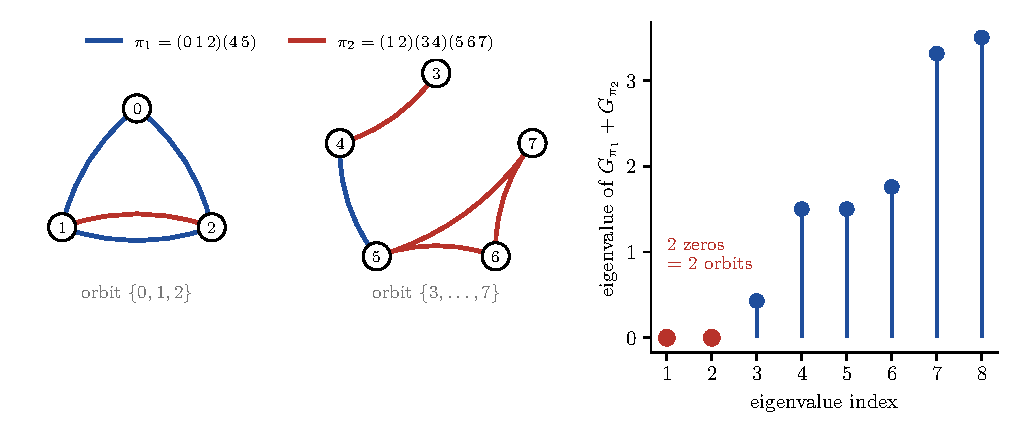
\includegraphics[width=.95\textwidth]{fig_schreier.pdf}
\caption{Two permutations of eight points read together. Left: the Schreier multigraph of the action, one colour per permutation; it has two orbits. Right: the spectrum of $G_{\pi_1}+G_{\pi_2}$, which is half the Laplacian of that graph. It has exactly two zero eigenvalues, one for each orbit, and the first positive eigenvalue is the spectral gap.}\label{fig:schreier}\end{figure}

\begin{proposition}[The fixed-scale entropy; T+V]\label{prop:entropy}
Let $K_U=G/2=(2I-U-U^*)/4$, normalised by the universal bound $0\le G\le 2I$ rather than by $\lambda_{\max}$, and let $h$ be the binary entropy. Then $\Tr h(K_U)=0$ if and only if $U^2=I$, that is, exactly on involutions. On a single $\ell$-cycle $S_\ell=\Tr h(K_U)$ satisfies $S_\ell/\ell\to\pi^{-1}\!\int_0^\pi h(\sin^2x)\,dx=2\ln2-1=0.3862943611\ldots$.
\end{proposition}
\begin{proof}
$h$ vanishes only at $0$ and $1$. An eigenphase $\phi$ of $U$ gives the eigenvalue $\sin^2(\phi/2)$ of $K_U$, which is $0$ or $1$ exactly when $e^{i\phi}=\pm1$. The limit is a Riemann sum.
\end{proof}
A normalisation by $\lambda_{\max}$ would not do: a 3-cycle has $G$-spectrum $\{0,\tfrac32,\tfrac32\}$, and its $\lambda_{\max}$-normalised entropy vanishes too, while $\Tr h(K_U)=2h(3/4)=1.1246702892\ldots$ [V].

\begin{proposition}[The finite-size deficit; T+V]\label{prop:zeta3}
Let $D_\ell=2\ln2-1-S_\ell/\ell$ on an $\ell$-cycle. Then
\[
D_\ell=\sum_{m\ge1,\ \ell\mid 2m}\frac{1}{m(4m^2-1)},
\]
so $D_\ell=D_{2\ell}$ for every odd $\ell$, and
\[
\ell^3D_\ell=\begin{cases}\displaystyle 2\sum_{t\ge1}\frac{1}{t\,(t^2-\ell^{-2})}\ \longrightarrow\ 2\zeta(3)=2.40411380632\ldots,&\ell\text{ even},\\[12pt] \displaystyle\sum_{t\ge1}\frac{1}{t\,(4t^2-\ell^{-2})}\ \longrightarrow\ \tfrac14\zeta(3)=0.30051422579\ldots,&\ell\text{ odd},\end{cases}
\]
with error $O(\ell^{-2})$ in both cases. More precisely, for every $\ell\ge2$ the corrections form a convergent series in odd zeta values:
\[
\ell^3D_\ell=\begin{cases}\displaystyle 2\sum_{r\ge0}\frac{\zeta(2r+3)}{\ell^{2r}}=2\zeta(3)+\frac{2\zeta(5)}{\ell^2}+\frac{2\zeta(7)}{\ell^4}+\cdots,&\ell\text{ even},\\[14pt] \displaystyle \frac14\sum_{r\ge0}\frac{\zeta(2r+3)}{4^r\ell^{2r}}=\frac{\zeta(3)}4+\frac{\zeta(5)}{16\,\ell^2}+\frac{\zeta(7)}{64\,\ell^4}+\cdots,&\ell\text{ odd}.\end{cases}
\]
\end{proposition}
\begin{proof}
On an $\ell$-cycle the eigenvalues of $K_U$ are $\sin^2(\pi j/\ell)$, $0\le j<\ell$, so $S_\ell=\sum_{j=0}^{\ell-1}f(j/\ell)$ with $f(x)=h(\sin^2\pi x)=-2\sin^2(\pi x)\ln|\sin\pi x|-2\cos^2(\pi x)\ln|\cos\pi x|$. Write $c_k=\cos(2\pi kx)$ and use the classical series
\[
-\ln|\sin\pi x|=\ln2+\sum_{k\ge1}\frac{c_k}{k},\qquad -\ln|\cos\pi x|=\ln2+\sum_{k\ge1}(-1)^k\frac{c_k}{k},
\]
together with $2\sin^2\pi x=1-c_1$ and $2\cos^2\pi x=1+c_1$. Then
\[
f=(1-c_1)\Big(\ln2+\sum_k\frac{c_k}{k}\Big)+(1+c_1)\Big(\ln2+\sum_k(-1)^k\frac{c_k}{k}\Big)
=2\ln2+\sum_{k\ \rm even}\frac{2c_k}{k}-\sum_{k\ \rm odd}\frac{2c_1c_k}{k}.
\]
With $2c_1c_k=c_{k+1}+c_{k-1}$, the last sum contributes $-1$ to the constant term (from $k=1$) and $-\big(\tfrac1{2m-1}+\tfrac1{2m+1}\big)c_{2m}$ for each $m\ge1$, while the even sum contributes $c_{2m}/m$. Since $\tfrac1m-\tfrac{4m}{4m^2-1}=-\tfrac1{m(4m^2-1)}$,
\[
f(x)=2\ln2-1-\sum_{m\ge1}\frac{\cos(4\pi mx)}{m(4m^2-1)},
\]
an absolutely convergent series. Its constant term is the integral of Proposition~\ref{prop:entropy}, and $f(0)=0$ is the partial-fraction identity $\sum_m 1/(m(4m^2-1))=2\ln2-1$. Summing over $x=j/\ell$, $\sum_{j=0}^{\ell-1}\cos(4\pi mj/\ell)$ is $\ell$ when $\ell\mid2m$ and $0$ otherwise, which gives the formula for $D_\ell$. If $\ell$ is odd, $\ell\mid2m$ means $\ell\mid m$, the same condition as $2\ell\mid2m$, so $D_\ell=D_{2\ell}$. Putting $m=\ell t$ for odd $\ell$ and $m=(\ell/2)t$ for even $\ell$ gives the two series for $\ell^3D_\ell$. For the expansion, write $\varepsilon=\ell^{-2}$. For even $\ell$, $\frac{2}{t(t^2-\varepsilon)}=\frac{2}{t^3}\sum_{r\ge0}(\varepsilon/t^2)^r$ with $\varepsilon/t^2\le\ell^{-2}<1$; for odd $\ell$, $\frac1{t(4t^2-\varepsilon)}=\frac1{4t^3}\sum_{r\ge0}(\varepsilon/4t^2)^r$. All terms are positive, so the sums over $t$ and $r$ may be exchanged, and $\sum_t t^{-(2r+3)}=\zeta(2r+3)$. The leading terms are the limits, and the next terms are $O(\ell^{-2})$.
\end{proof}
The parity split has a plain reading: an even cycle has the eigenphase $\pi$, where $\sin^2$ reaches $1$ and $h$ has its second zero, and an odd cycle does not. Numerically, the direct sums agree with the exact series to $10^{-29}$ relative for $\ell=2,\dots,39$ and at $\ell=63,64,126,127,1000,1001,4096,4097$, and $D_{63}-D_{126}=-1.7\times10^{-41}$ at 40-digit working precision (script \texttt{K3-V4-DEFICIT}); the zeta-value expansion matches the direct sums to $1.4\times10^{-33}$ relative for $\ell$ from $2$ to $256$ (script \texttt{K3-V5-CHECKS}) [V].

The cycle-by-cycle results have a global counterpart that holds for every permutation at once.
\begin{proposition}[The entropy is controlled by the Hamming defect; T+V]\label{prop:entropybound}
For every permutation matrix $U$ of degree $n$,
\[
\frac1n\Tr K_U=\frac12\,\dH(U,I),\qquad 0\le\frac1n\,S(U)\le h\!\Big(\frac{\dH(U,I)}2\Big),\qquad S(U)=\Tr h(K_U),
\]
and for two permutations $U,V$ the same holds with $U^*V$ in place of $U$ and $\dH(U,V)$ in place of $\dH(U,I)$.
\end{proposition}
\begin{proof}
$\Tr G_U=n-\Tr U$, and $\Tr U$ is the number of fixed points, so $\Tr G_U=n\,\dH(U,I)$ and $\Tr K_U=\tfrac n2\dH(U,I)$. The eigenvalues of $K_U$ lie in $[0,1]$, and $h$ is concave there, so by Jensen's inequality the mean of $h$ over the $n$ eigenvalues is at most $h$ of their mean. The second statement follows because $\dH(U,V)=\dH(U^*V,I)$.
\end{proof}
So the normalised entropy tends to zero whenever the Hamming defect does, for every permutation, not only along the cycles computed above. The bound behaves like $\tfrac{d}{2}\log\tfrac2d$ for small $d=\dH$: the entropy is continuous at the identity but not Lipschitz there. Equality holds only at the identity: $h$ is strictly concave, so equality in Jensen's inequality needs all eigenvalues of $K_U$ equal, and every cycle contributes the eigenvalue $0$. Script \texttt{K3-V6-CHECKS} finds no violation over $2000$ random permutations [V].

\begin{figure}[t]\centering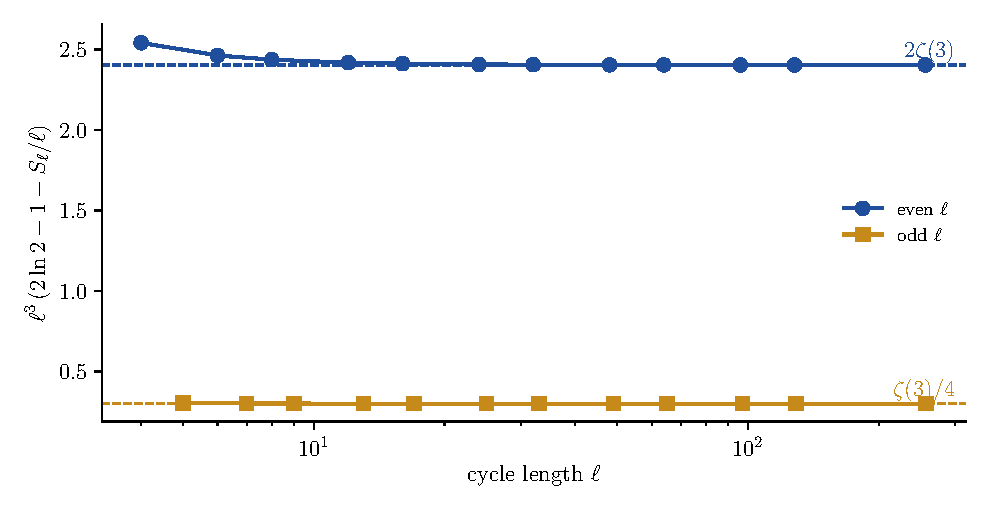
\includegraphics[width=.85\textwidth]{fig_entropy_deficit.pdf}
\caption{The finite-size deficit of the fixed-scale entropy on an $\ell$-cycle, scaled by $\ell^3$. Points are direct sums; dashed lines are the limits $2\zeta(3)$ for even cycles and $\zeta(3)/4$ for odd cycles proved in Proposition~\ref{prop:zeta3}. The odd curve is the even curve read at $2\ell$ and divided by $8$, because $D_\ell=D_{2\ell}$ for odd $\ell$.}\label{fig:deficit}\end{figure}

\subsection{The Hamming metric is a squared distance between graph projectors}
The identities in this subsection hold for every finite unitary $U$. Put
\[
Q_U=\tfrac1{\sqrt2}\begin{pmatrix}I\\U\end{pmatrix},\qquad Q_I=\tfrac1{\sqrt2}\begin{pmatrix}I\\I\end{pmatrix},\qquad P_U=Q_UQ_U^*,\qquad P_I=Q_IQ_I^*,
\]
the orthogonal projectors onto the graphs of $U$ and of $I$.
\begin{proposition}[T+V]\label{prop:graph}
$Q_U^*(I-P_I)Q_U=K_U=G/2$. Hence the eigenvalues of $K_U$ are the squared sines of the principal angles between $\mathrm{graph}(I)$ and $\mathrm{graph}(U)$. For permutation matrices $U,V$ of degree $n$,
\[
\dH(U,V)=\frac1n\,\|P_U-P_V\|_F^2=\frac2n\sum_{j=1}^n\sin^2\theta_j,
\]
where $\theta_j$ are the principal angles between $\mathrm{graph}(U)$ and $\mathrm{graph}(V)$, and $\sin^2\theta_j=\sin^2(\phi_j/2)$ for the eigenphases $\phi_j$ of $U^*V$. So Hamming distance is twice the mean squared sine of the principal angles between the two graphs, and since $\sin\theta\le\theta\le\tfrac\pi2\sin\theta$ on $[0,\tfrac\pi2]$,
\[
\frac{\dH(U,V)}2\;\le\;\frac1n\sum_{j=1}^n\theta_j^2\;\le\;\frac{\pi^2}{8}\,\dH(U,V).
\]
Hamming convergence of permutations is therefore equivalent, with these constants, to convergence of their graph subspaces in the Grassmannian geodesic distance. The upper constant is attained by a transposition, whose angle is $\pi/2$.
\end{proposition}
\begin{proof}
$Q_I^*Q_U=(I+U)/2$, so $Q_U^*(I-P_I)Q_U=I-\tfrac14(I+U^*)(I+U)=\tfrac14(2I-U-U^*)$, and the principal angles are read from the singular values of $Q_I^*Q_U$. For the second identity, $P_U-P_V=\tfrac12\begin{pmatrix}0&U^*-V^*\\U-V&0\end{pmatrix}$, so $\|P_U-P_V\|_F^2=\tfrac12\|U-V\|_F^2$, and $\|U-V\|_F^2=2n\,\dH(U,V)$ for permutation matrices. For two projectors of equal rank $n$, $\|P_U-P_V\|_F^2=2\sum_j\sin^2\theta_j$. Finally $Q_U^*Q_V=\tfrac12(I+U^*V)$ has singular values $|1+e^{i\phi_j}|/2=|\cos(\phi_j/2)|=\cos\theta_j$. The angle form was checked on 300 random pairs of permutations of up to 12 points, to $5\times10^{-15}$ (script \texttt{K3-V5-CHECKS}), and the two-sided bound on 2000 random pairs (script \texttt{K3-V6-CHECKS}) [V].
\end{proof}
On the complement $\mathcal H_0$ of the $+1$ eigenspace of $U$ the inverse Cayley transform $Z=(I+U)(I-U)^{-1}$ exists, with eigenvalue $i\cot(\phi/2)$ at $e^{i\phi}\ne1$. With $X=-iZ=X^*$,
\[
U=(Z-I)(Z+I)^{-1},\qquad K_U=(I+X^2)^{-1}\ \text{on }\mathcal H_0,\qquad \sin^2\theta=\sin^2(\phi/2)=\frac1{1+\cot^2(\phi/2)} .
\]
So the resolvability threshold $\sin^2\theta\ge\varepsilon$ becomes the spectral bound $|X|\le\sqrt{\varepsilon^{-1}-1}$. The $+1$ eigenspace is a pole of this chart, not lost information, and its projector is kept separately; and since $Z^*=-Z$, the unitary sits on the lossless boundary of the passive Smith domain. These are coordinate conversions, checked on 57 permutations of $2$ to $20$ points with residuals below $6.4\times10^{-16}$ for the projector identities and $5.1\times10^{-14}$ for the Cayley chart [V]. They are not a physical law.

\subsection{A fixed probe separates isospectral defects}
Take $\pi_a=(01)(23)$ and $\pi_b=(02)(13)$ on four labelled points. Their Gram spectra are both $\{0,0,2,2\}$, their Hamming defects are both $1$, and every scalar spectral functional agrees; for instance $\det(I+G_a)=\det(I+G_b)=9$. Hold the probe $b=(e_0+e_1)/\sqrt2$ fixed. Then
\[
m_b(G)=b^*(I+G)^{-1}b:\qquad m_b(G_a)=1,\qquad m_b(G_b)=\tfrac23,
\]
because $b$ lies in the kernel of $G_a$ and splits equally between the eigenvalues $0$ and $2$ of $G_b$. Eliminating every other coordinate by the Schur complement of $I+G$ leaves the scalar boundary coefficient $z_b=1/m_b$, and the Smith normalisation gives $\Gamma_b=(z_b-1)/(z_b+1)=(1-m_b)/(1+m_b)$, which is $0$ for $\pi_a$ and $\tfrac15$ for $\pi_b$ [T+V, exact rational]. By the matrix determinant lemma, for $c>0$,
\[
\left.\frac{d}{dt}\log\det\big(cI+G+t\,bb^*\big)\right|_{t=0}=b^*(cI+G)^{-1}b,
\]
so a scalar log-determinant of an isospectral family cannot distinguish probe orientation, while a family of probe insertions can. The example is one case of a general statement.
\begin{proposition}[What a fixed probe reads; T+V]\label{prop:probe}
Let $G=G^*\ge0$ have spectral decomposition $G=\sum_j\lambda_jP_j$, fix a vector $b$, and put $m_b(c;G)=b^*(cI+G)^{-1}b$ for $c>0$. Then
\[
m_b(c;G)=\sum_j\frac{\|P_jb\|^2}{c+\lambda_j}=\int\frac{d\mu_b(\lambda)}{c+\lambda},\qquad \mu_b=\sum_j\|P_jb\|^2\,\delta_{\lambda_j},
\]
and the function $c\mapsto m_b(c;G)$ on $c>0$ determines the spectral measure $\mu_b$ of $G$ seen by $b$.
\end{proposition}
\begin{proof}
The formula is the spectral decomposition of $(cI+G)^{-1}$. The function is a rational function of $c$ whose partial-fraction decomposition has poles at $c=-\lambda_j$ with residues $\|P_jb\|^2$, and a partial-fraction decomposition is unique, so the function determines every pair $(\lambda_j,\|P_jb\|^2)$ with nonzero weight; $m_b$ is the Stieltjes transform of $\mu_b$. Differentiating under the finite sum, $(-1)^rm_b^{(r)}(c)=r!\int(c+\lambda)^{-r-1}d\mu_b(\lambda)\ge0$, so $m_b$ is completely monotone on $c>0$.
\end{proof}
Eigenvalues alone fix the support of $\mu_b$ but not its weights; the weights record where the eigenspaces sit relative to the probe. In the example, $\mu_b=\delta_0$ for $\pi_a$ and $\mu_b=\tfrac12\delta_0+\tfrac12\delta_2$ for $\pi_b$ (script \texttt{K3-V5-CHECKS}) [V]: same spectrum, different measure. This is a constructed finite response, not a measurement and not a claim that graph entries are an impedance.

Read together with the winding of the earlier attempt \cite{trace}: the Exel--Loring winding of a commutator is rigid and jumps under the local surgery Hamming forgives; the regularised torsion is Lipschitz in Hamming and varies smoothly under the same surgery; the displacement Gram and its graph-projector form read a defect that is \emph{given}, exactly and down to its arrangement, but forbid nothing, and the entropy built from it is bounded by $h(\dH/2)$ and so vanishes with the defect; summed over a family, the same Gram is the Schreier Laplacian of the action, whose gap is the expansion that the known non-sofic constructions use; and the fixed probe recovers what a scalar spectrum discards without becoming an obstruction. The constant of Sections 3 and 4 is the only quantity here that both lives natively in the metric and produces a number, and it does so by an incidence count.

\section{Formal verification}\label{sec:lean}
The Lean 4 library (v4.34.1, Mathlib v4.34.1) in the public repository \cite{lean} holds 66 theorems in three modules, with no \texttt{sorry} and no \texttt{native\_decide}. Every module is replayed by an independent kernel checker, the axioms of every named theorem are audited (only \texttt{propext}, \texttt{Classical.choice} and \texttt{Quot.sound} appear), and four deliberately false statements must fail on every build. The gauge exhaustions run in the kernel (\texttt{decide +kernel}); for $k=6,7,8$ a branch-and-bound search is used with its soundness proved (\texttt{search\_sound}), split into kernel-checked pieces at $k=7,8$.

\begin{itemize}
\item The five witnesses of Theorem~\ref{thm:small}, with the exact defect, every gauge costing at least $D$, and $D$ attained (\texttt{witness\_k4} to \texttt{witness\_k8}); that fixing the root gauge loses nothing (\texttt{gauge\_lower}); the $k=4$ mechanism (\texttt{k4\_mechanism}); the Gram formula of Theorem~\ref{thm:gram} (\texttt{disp\_gram}).
\item The equality case of Corollary~\ref{cor:equality} on every witness: each star gauge costs exactly $D$ and the star costs add up to $3N$ (\texttt{stars\_k4} to \texttt{stars\_k8}, \texttt{stars\_r8}).
\item The parity retraction of Theorem~\ref{thm:all}, for every $k$: $r$ is the sign map read in $\{\Id,t\}$, a homomorphism that never moves more points, and retracting any $\Sym(3)$ gauge of a binary cochain never raises its cost (\texttt{retract\_cost}, \texttt{binary\_gauge\_suffices}).
\item Lemma~\ref{lem:rep} for every cochain, every $k$ and every $q$: the defect is multiplied by $q^3$ (\texttt{rep\_defect}), a cluster-constant gauge costs $q^2$ times its seed cost (\texttt{rep\_attain}), and every gauge costs at least $q^2D$ by the count over the $q^k$ sections (\texttt{rep\_lower}); and Corollary~\ref{cor:mult4} for every $q$: the replicated seed has $N=8q^3$ and gauge minimum exactly $6q^2$ (\texttt{rep\_seed}). The replicated $K_8$ is also checked exhaustively (\texttt{witness\_r8}).
\item Proposition~\ref{prop:crossdeg} on the seed: against comparison permutations of degree 2, 3 and 4 the cheapest repair is $10/3$, $2$ and $3$ (\texttt{cross\_degree\_seed}).
\end{itemize}

Not formalised: the lower bound of Proposition~\ref{prop:cl} for general $k$ (proved in Section~\ref{sec:bound}); Kozlov's theorem for $\F_2$ and the assembly of the three cases into Theorem~\ref{thm:all}; the cross-degree baselines beyond the seed; the subgroup minima of Proposition~\ref{prop:k4}; the cycle-Laplacian eigenvalues (in Lean only the rewriting $2-2\cos2x=4\sin^2x$ is proved); and everything in Section~\ref{sec:readings} beyond Theorem~\ref{thm:gram}. The torsion constants quoted in Proposition~\ref{prop:torsion} were measured in the August session and their own scripts are not part of this package; the identity they illustrate is replayed independently by \texttt{K3-V7-TORSION}, which is. Every other computation in this paper is shipped in Appendix~\ref{sec:gates}.

\section{Relation to the soficity problem}
Chapman--Lubotzky's programme asks for positive \emph{permutation} cocycle Cheeger constants on bounded-degree complexes, such as quotients of Bruhat--Tits buildings, from which non-sofic groups would follow \cite[Section~6.1]{CL2}. The complete complexes are the calibration platform of that programme, and Theorem~\ref{thm:all} settles the calibration: the elementary bound is the truth for permutation coefficients at every $k$, including the powers of two where it is not the truth for $\F_2$. As of 8 October 2026, non-sofic groups exist by other routes: from property (T) expanders and the Kun--Thom extension graphs \cite{Astra,FF,KT,AT}, and, in unrefereed manuscripts of October 2026, from counterexamples to Kaplansky's direct-finiteness conjecture in characteristic two \cite{OAIkap1,OAIkap2} through Elek--Szab\'o \cite{ES}. A companion manuscript constructs bounded-degree coboundary expanders over $\F_2$ in every dimension \cite{OAIexp}; the permutation-coefficient case the programme needs remains open. None of this is used in the proofs above, nothing here bears on the existence of non-sofic groups, and no priority is claimed in that direction.

\section*{Acknowledgements}
The balanced-replication argument, the parity retraction, the cross-degree check, the graph-projector and Cayley dictionary and the isospectral probe were developed with AI assistance (ChatGPT, in the working addendum COMPLETE-COMPLEX-BRIDGE-01 of 5 September 2026), and independently re-derived and verified with Claude, which also wrote the Lean library and the checks for this version. The structure of the Lean replication module was drafted by Grok (xAI) and completed with Claude. AI readings of the previous version suggested writing out the proof of Proposition~\ref{prop:cl}, the equality case, the finite form of the replication count, the closed form and zeta-value expansion of Proposition~\ref{prop:zeta3}, the general probe statement, the principal-angle form of the graph-projector identity and its two-sided bound, the global entropy bound, and the positive-aggregate statement, whose reading as a Schreier Laplacian was added here; each was checked here before inclusion. No statement rests on an AI's say-so: every computation is shipped as an executable script, and the witnesses are kernel-checked.

\renewcommand{\refname}{Sources}
\begin{thebibliography}{99}\small
\bibitem{CL1} M.~Chapman and A.~Lubotzky, \emph{Stability of homomorphisms, coverings and cocycles I: equivalence}, Eur.\ J.\ Math.\ 11 (2025), art.\ 13; arXiv:2310.17474.
\bibitem{CL2} M.~Chapman and A.~Lubotzky, \emph{Stability of homomorphisms, coverings and cocycles II: examples, applications and open problems}, Adv.\ Math.\ 463 (2025), 110117; arXiv:2311.06706. Proposition 3.2 is the bound; footnote 2 is $h_1(\cdot,\Sym)\le h_1(\cdot,\F_2)$.
\bibitem{LM} N.~Linial and R.~Meshulam, \emph{Homological connectivity of random 2-complexes}, Combinatorica 26 (2006) 475--487.
\bibitem{MW} R.~Meshulam and N.~Wallach, \emph{Homological connectivity of random $k$-dimensional complexes}, Random Structures Algorithms 34 (2009) 408--417.
\bibitem{Koz} D.~N.~Kozlov, \emph{The first Cheeger constant of a simplex}, Graphs Combin.\ 33 (2017); arXiv:1610.07136. Theorem 4.2 and Corollary 4.3: $h(n)=n/3$ for $n=c(2t+1)$, $t\ge1$, hence whenever $n$ is not a power of two. Theorem 4.6: $h(n)-n/3\le 4n/(3(n^2-8))$ for $n=2^d$, $d\ge3$. Section 4.2: $h(4)=2$, $h(8)=8/3+4/21$.
\bibitem{DD} Y.~Dikstein and I.~Dinur, \emph{Swap cosystolic expansion}, arXiv:2312.15325, Section~6.
\bibitem{DS} D.~Cvetkovi\'{c}, M.~Doob and H.~Sachs, \emph{Spectra of Graphs}, 3rd ed., 1995; E.~R.~van Dam and W.~H.~Haemers, \emph{Which graphs are determined by their spectrum?}, Linear Algebra Appl.\ 373 (2003). Regular graphs of degree at most two are determined by their spectrum.
\bibitem{SW} D.~S.~Silver and S.~G.~Williams, \emph{Twisted Alexander polynomials detect the unknot}, Algebr.\ Geom.\ Topol.\ 6 (2006) 1893--1901; the twisted invariant as in Wada, Topology 33 (1994) 241--256.
\bibitem{ES} G.~Elek and E.~Szab\'o, \emph{Sofic groups and direct finiteness}, J.\ Algebra 280 (2004) 426--434.
\bibitem{Astra} OpenAI, \emph{Ten advances in mathematics and theoretical computer science}, 1 August 2026; github.com/openai/ten-proofs.
\bibitem{FF} F.~Fournier-Facio, \emph{A torsion-free non-sofic group}, arXiv:2608.02025.
\bibitem{KT} G.~Kun and A.~Thom, arXiv:2608.06222.
\bibitem{AT} V.~Alekseev and A.~Thom, arXiv:2608.05362.
\bibitem{OAIexp} OpenAI, \emph{Bounded-degree coboundary expanders in every dimension}, manuscript dated 24 September 2026, in github.com/openai/math (released 6--7 October 2026). Unrefereed.
\bibitem{OAIkap1} OpenAI, \emph{A counterexample to Kaplansky's direct-finiteness conjecture in characteristic two}, manuscript dated 23 September 2026, in github.com/openai/math. Unrefereed.
\bibitem{OAIkap2} OpenAI, \emph{A torsion-free group algebra that is not directly finite}, manuscript dated 4 October 2026, in github.com/openai/math. Unrefereed.
\bibitem{trace} J.~Beasley, \emph{The Soficity Trace: what was tried, what failed, what survived, and what it cost}, working record, 23 August 2026.
\bibitem{EL} R.~Exel and T.~A.~Loring, \emph{Invariants of almost commuting unitaries}, J.\ Funct.\ Anal.\ 95 (1991) 364--376.
\bibitem{Kun} G.~Kun, \emph{On sofic approximations of property (T) groups}, arXiv:1606.04471.
\bibitem{lean} J.~Beasley, \emph{coboundary-k3-lean}, github.com/dicipler-pixel/coboundary-k3-lean, commit \texttt{391104b} (8 October 2026).
\end{thebibliography}

\appendix
\section{The witnesses}\label{sec:witnesses}
Vertices are $0,\dots,k-1$; permutations of $\{0,1,2\}$ are written one-line; every edge not listed carries the identity; $(u,v)$ with $u<v$ is the value on the oriented edge $u\to v$. Each computed witness is given in gauged form (the residual after the minimising coboundary), so the listed edges are exactly the support that costs $D$.
\begin{itemize}\small\renewcommand{\labelitemi}{--}
\item $k=4$ ($N/D=8/6$): $(1,2)\mapsto(0\,2\,1)$, $(1,3)\mapsto(1\,0\,2)$, $(2,3)\mapsto(2\,1\,0)$.
\item $k=5$ ($10/6$): $(0,1),(1,2),(2,3)\mapsto(1\,0\,2)$.
\item $k=6$ ($36/18$): $(0,1),(1,3)\mapsto(1\,2\,0)$; $(0,3),(0,4),(1,5),(4,5)\mapsto(2\,0\,1)$.
\item $k=7$ ($28/12$): $(0,1),\allowbreak(0,3),\allowbreak(0,4),\allowbreak(1,2),\allowbreak(1,5),\allowbreak(2,3)\mapsto(1\,0\,2)$.
\item $k=8$ ($72/27$): $(0,1),\allowbreak(0,7),\allowbreak(1,2),\allowbreak(2,5),\allowbreak(2,7)\mapsto(0\,2\,1)$; $(1,3),\allowbreak(1,4),\allowbreak(1,6),\allowbreak(3,7)\mapsto(1\,0\,2)$; $(0,4),\allowbreak(2,3),\allowbreak(2,4)\mapsto(2\,1\,0)$; $(4,7)\mapsto(2\,0\,1)$.
\item $k=8$, replicated seed ($64/24$): clusters $\{0,1\},\{2,3\},\{4,5\},\{6,7\}$; every edge between $\{2,3\}$ and $\{4,5\}\mapsto(1\,0\,2)$, between $\{2,3\}$ and $\{6,7\}\mapsto(2\,1\,0)$, between $\{4,5\}$ and $\{6,7\}\mapsto(0\,2\,1)$.
\end{itemize}
For the $(72,27)$ witness the ungauged cochain as found by the search has 22 non-identity edges; it is the input to the verification script below, which gauges it to the residual above.

\section{The gates, as run}\label{sec:gates}
\subsection*{Independent verification of every computed witness}
\lstinputlisting{COBND-WITNESS-VERIFY-ALL.py}
\subsection*{The replication lemma at \texorpdfstring{$q=2$}{q=2}, exhaustive}
\lstinputlisting{REPLICATION-CHECK-01.py}
\subsection*{The \texorpdfstring{$k=8$}{k=8} search}
\lstinputlisting{COBND-WITNESS-08b.py}
\subsection*{\texorpdfstring{$k=4$}{k=4} by coefficient subgroup}
\lstinputlisting{k4sub.py}
\subsection*{Retraction, cross-degree, Gram, projector, Cayley, entropy and probe checks}
\lstinputlisting{COMPLETE-COMPLEX-BRIDGE-01.py}
\subsection*{Flat profiles, cycle recovery and the \texorpdfstring{$\zeta(3)$}{zeta(3)} deficit}
\lstinputlisting{K3-V3-CHECKS.py}
\subsection*{The closed form of the deficit}
\lstinputlisting{K3-V4-DEFICIT.py}
\subsection*{Zeta expansion, probe measure and principal angles}
\lstinputlisting{K3-V5-CHECKS.py}
\subsection*{Entropy bound, angle sandwich, Schreier aggregates and probe bins}
\lstinputlisting{K3-V6-CHECKS.py}
\subsection*{The torsion identity, replayed}
\lstinputlisting{K3-V7-TORSION.py}
\subsection*{The equality case on every witness}
\lstinputlisting{K3-V4-STAR.py}
\end{document}
